\documentclass{article}
\usepackage[utf8]{inputenc}
\usepackage{hyperref}

\usepackage{url}
\usepackage{listings}
\usepackage[pass]{geometry}
% \usepackage{vmargin}
\usepackage{fancyhdr}
\usepackage{amsmath}
\usepackage{amsfonts,amssymb,amsthm,cite,float,graphicx}
\graphicspath{ {images/} }
% \usepackage[tight,footnotesize]{subfigure}
\usepackage[usenames]{color}
\usepackage{algorithm,algorithmic}
\usepackage{natbib}    % this package seems sensitive to location placement
\usepackage{graphicx}
\usepackage{caption}
\usepackage{subcaption}
\usepackage{multicol}
\usepackage{float}
\usepackage{mathtools}


\title{Simplified Hodgkin-Huxley Model}
\author{Faris Sbahi and Stuart Ki}
\date{April 2017}

\begin{document}

\maketitle

\section{Introduction}

Alan Lloyd Hodgkin and Andrew Huxley, in 1963, won the Noble Prize in Physiology and Medicine for their work developing the Hodgkin-Huxley Equations, equations that modeled to incredible accuracy the propagation of action potentials through a squid axon. 

\section{Premises of the Hodgkin-Huxley Model}

The Hodgkin-Huxley model models the cell membrane as a simple circuit. 

\begin{figure}[h]
    \centering
    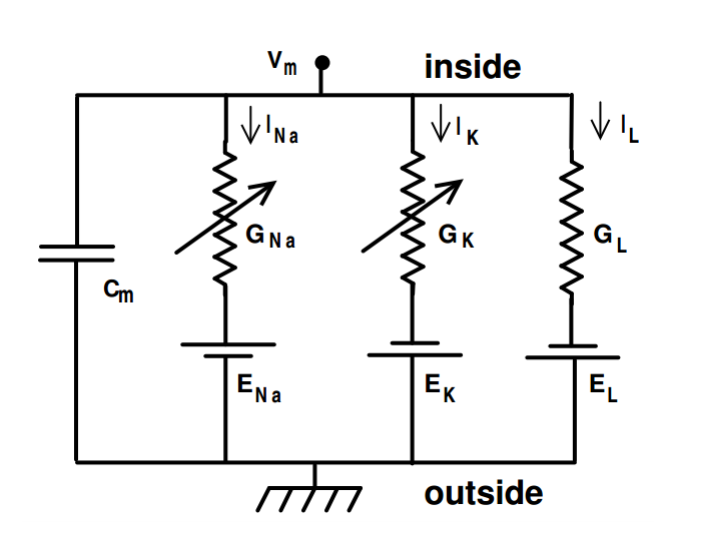
\includegraphics[scale=0.5]{hhmodel}
    \caption{Hodgkin-Huxley Circuit}
    \label{fig:my_label}
\end{figure}


Two voltage-dependent sodium and potassium channels allow the ions to flow through the membrane. The membrane has a capacitance indicated by $c_m$. Additionally, the sodium and potassium channels have a conductance parameter $G_{Na}$ and $G_K$, as well as a leakage conductance as shown. These conductances can be modeled by various functions as will be shown later, and model the buildup in the passage of ions that create the action potential. The circuit is in parallel to mimic the axon. 

Using classic current conservation in a circuit, and adding the parameter of an external current $I_{ext}$, we can derive the current equation for the cell.

\begin{equation}
    c_m\frac{dV_m}{dt} + I_{ion} = I_{ext}
\end{equation}

In our particular model, we will assume that $G_L$ is constant and the capacitance $c_m$ as well. $V_m$ is the potential within the cell mebrane, and $I_{ion}$ is the net ionic current within the cell.

The derivation of each ionic current through the different channels depends on the conductance parameter times the driving potential.

\begin{equation}
    I_{ion} = G_{ion}(V_{m}-E_{ion})
\end{equation}

Conductance is modeled in a certain way. The physical meaning of conductance is the probability that the channels that the ions pass through will be considered open, or when the gates that the ions can pass through are all permissive in that particular ion channel. This is dependent on the voltage of the cell membrane. 

Hodgkin and Huxley used three different types of gates to model the conductance channels. Using, $m$, $h$, and $n$ as different types of gates, $G_{Na}$ and $G_K$ are modeled as followed.
\begin{equation}
    G_{Na} = \bar{G}_{Na}m^3h
\end{equation}
\begin{equation}
    G_{K} = \bar{G}_{K}n^4
\end{equation}

Where $m$, $h$, and $n$ follow the following differential equation, which is derived on the open fraction of gates, $p$:

\begin{equation}
    \frac{dp}{dt} = a(V)(1-p) - b(V)p
\end{equation}

Hodgkin and Huxley discovered that as they kept the voltage constant, the conductance of the channels increased steadily to a maximum value. 

\begin{equation}
    \frac{dp}{dt} = \frac{p_{\infty}(V)-p}{\tau_p(V)}
\end{equation}

Where $p_{\infty}(V)$ is the steady state value at an given voltage and ${\tau_p}(V)$ are time constants of response of the gates. The combined system of differential equations is shown in the next section. 

\section{Deriving a Reduced-State Model}

Evidently, the state variables for the model are $V$, $m$, $h$, and $n$. Hence, we can write

\begin{align*}
    C\frac{dV}{dt} &= I_{ext} -\bar{G}_{Na}m^3h(V-E_{Na}) -\bar{G}_{K}n^4(V-E_{K})  -\bar{G}_{L}m^3h(V-E_{L}) \\
    \frac{dm}{dt} &= \frac{m_{\infty}(V)-m}{\tau_m(V)} \\
    \frac{dh}{dt} &= \frac{h_{\infty}(V)-h}{\tau_h(V)} \\
    \frac{dn}{dt} &= \frac{n_{\infty}(V)-n}{\tau_n(V)} 
\end{align*}

While analyzing a four-dimensional nonlinear system is certainly feasible, it is difficult to then visualize our results. Furthermore, the number of combinations of parameters grows exponentially with each new parameter introduced. Hence, we seek to reduce the number of state variables in our model to gain better insights into our model both visually and analytically. 

\begin{figure}[h]
\centering
\begin{subfigure}{.5\textwidth}
	\centering
	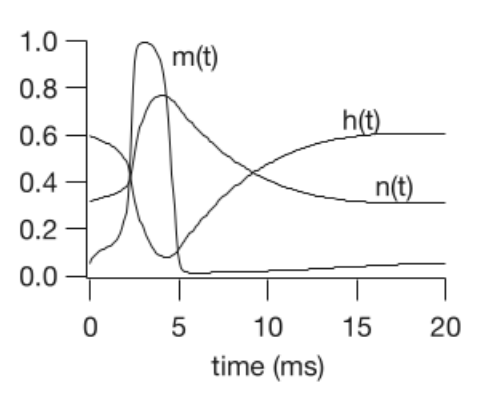
\includegraphics[height=5cm]{keener1.png}
	\caption{Gate Variables}
\end{subfigure}%
\begin{subfigure}{.5\textwidth}
	\centering
	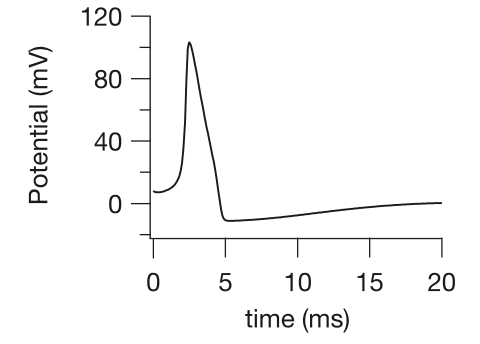
\includegraphics[height=5cm]{keener2.png}
	\caption{Action Potential}
\end{subfigure}
	\caption{Dynamics of Action Potential on Shared Time-Scale (ms)}
	\label{fig:keen}
\end{figure}


Firstly, it has been observed empirically that the time constants, $\tau_i$ vary widely between these equations. In fact, reasonable estimates are $\tau_m \approx 0.4 ms$, $\tau_h \approx 8 ms$, and $\tau_n \approx 5 ms$.\cite{monster} Recall that $\tau_m$ is a measure of the speed with which $m$ converges to its steady state value $m_\infty$. Therefore, it may be a reasonable assumption to assume that $\tau_m$ is so fast compared to the other parameters that $m = m_\infty$. Then, we can either take $n$ or $h$ to be constant which would then give us a two-dimensional nonlinear system. Since $h$ fluctuates over the largest time-scale, we'll take it to be some constant $\bar{h}$. As a result, we have 

\begin{align*}
        C\frac{dV}{dt} &= I_{ext} -\bar{G}_{Na}m_\infty^3\bar{h}(V-E_{Na}) -\bar{G}_{K}n^4(V-E_{K})  -\bar{G}_{L}(V-E_{L}) \\
    \frac{dn}{dt} &= \frac{n_{\infty}-n}{\tau_n} 
\end{align*}

The assumption of taking $h$ to be constant can be judged visually in Figure \ref{fig:keen}, borrowed from Keener and Sneyd\cite{keener}. We'll develop this assumption further in a later section.

\section{Improving our Model}

In our previous simplification, taking $m$ to converge infinitely fast to $m_\infty$ lent itself as a natural assumption due to its magnitude in speed relative to the other convergence speeds. However, taking $h$ to be constant seemed to be a shakier assumption, which was evaluated using Figure \ref{fig:keen}. However, one may have also observed, from the same figure, that there was some parity over $\approx 0.5$ that could be used. In other words, one could take the improved assumption that $n + h = 1$ which would imply that we could substitute $1 - n$ for $h$ rather than assuming that it is constant.

Evidently, this would give us

\begin{align*}
        C\frac{dV}{dt} &= I_{ext}-\bar{G}_{Na}m_\infty^3(1-n)(V-E_{Na}) -\bar{G}_{K}n^4(V-E_{K})  -\bar{G}_{L}(V-E_{L}) \\
    \frac{dn}{dt} &= \frac{n_{\infty}-n}{\tau_n} 
\end{align*}

We can then begin our analysis the usual way, finding the null-clines to then find the fixed points. Hence, $\frac{dn}{dt}=0$ when $n_{\infty}=n$ and $\frac{dV}{dt}=0$ is satisfied when

\begin{align*}
        V &= \frac{\bar{G}_{Na}m_\infty^3(1-n)E_{Na}+\bar{G}_Kn^4E_K + G_LE_L + I_{ext}}{G_L + \bar{G}_{Na}m^3(1-n)+ \bar{G}_Kn^4}
\end{align*}

Note that $I_{ext}$ shifts up the $V$ null-cline monotonically.

\section{Conclusion}

\bibliography{nonlinear}
\bibliographystyle{plain}
\nocite{*}

\end{document}
